\chapter{Two level system}
\label{chap:twoLevelSystem}
Before we move to more complicated Hamiltonian model, we investigate a simple two level system. To understand the general behavior of fidelity on Hamiltonian spectrum, two analytically solvable drivings — \emph{geodesic} and \emph{linear} — is investigated.

\section{Hamiltonian}
Let's have a Hamiltonian
\begin{equation}
    \HH(t)=\begin{pmatrix}
        \Omega(t)&\Delta(t)\\
        \Delta(t)&-\Omega(t)
    \end{pmatrix}
\end{equation}
for $\Omega: \R^+\rightarrow \R$, $\Delta: \R^+\rightarrow \R$ and time $t$. Its spectrum is
\begin{equation}
    E_1(t)=-E_0(t)= \sqrt{\Omega^2(t)+\Delta^2(t)}
    \label{eq:energy}
\end{equation}
and using the eigenbasis
\begin{equation}
    \mathcal{B}\coloneqq \left\{
        \ket{0}\equiv\begin{pmatrix}
                1\\0
            \end{pmatrix},
        \ket{1}\equiv\begin{pmatrix}
            0\\1
        \end{pmatrix} \right\},
    \label{eq:eigenbasisDef}
\end{equation}
the eigenvectors  can be written as 
\begin{equation}
\ket{0(t)}=N_+ \begin{pmatrix}
    1\\ \frac{E_0(t)+\Omega(t)}{\Delta(t)}
\end{pmatrix},\quad \ket{1(t)}=N_-\begin{pmatrix}
    1\\ \frac{E_1(t)+\Omega(t)}{\Delta(t)}
   \end{pmatrix}
   \label{eq:eigenvectors}
\end{equation}
for normalization constants $N_\pm\coloneqq\left(\left(\frac{\pm E_0(t)+\Omega(t)}{\Delta(t)}\right)^2+1\right)^{-1/2}$. Notice that the eigenbases differ in time, but are described using constant basis $\mathcal B$, which forms an eigenbasis at time $t=0$.

The goal is to find \emph{fidelity} $F_{\mathcal J}(t)\coloneqq |\braket{0(t)|\psi(t)}|^2$ of different driving protocols \begin{equation}
    \mathcal J\coloneqq\{\llambda(t)|t\in[0,T],\; \llambda\in \mathcal U\} \subset \R^N.
\end{equation}
For this we need to solve time Schr\"odinger equation
\begin{equation}
    \HH(t)\ket{\psi(t)}=i\frac{\d}{\d t}\ket{\psi(t)}
\end{equation}
with time varying Hamiltonian $\HH(\llambda(t))\eqqcolon \HH(t)$ and $\llambda$ on path $\mathcal J$. For 2-dimentional system with 
\begin{equation}
    \ket{\psi(t)}\eqqcolon \begin{pmatrix}
         a(t) \\
         b(t)    
    \end{pmatrix},
\end{equation}
we get the system of \emph{two coupled differentials equations of the first order with non-constant coefficients}
\begin{align}
    \Omega(t)a(t)+\Delta(t)b(t)&=i\dot a(t)\label{eq:a1}\\
    \Delta(t)a(t)-\Omega(t)b(t)&=i\dot b(t)
    \label{eq:a2}
\end{align}
with normalization
\begin{equation}
    a^2(t)+b^2(t)=1, \quad \forall t\in [0,T].
    \label{eq:normalizationCondition}
\end{equation}
and initial value 
\begin{equation}
    \begin{pmatrix}
        a(0)\\b(0)
    \end{pmatrix} = \ket{0(0)}.
\end{equation}















\section{Harmonic oscillator correspondence}
Coupled Equations \ref{eq:a1}, \ref{eq:a2} have no general analytical solution, with an exception to a few easy protocols $\mathcal J$. Before moving to some of these special cases, let's analyze this coupled system of equations generally.

N-dimensional Schr\"odinger equation can be rewritten to \emph{one differential equation of N$^{th}$ order with non-constant coefficients}. In our two-dimensional case, this equation corresponds to \emph{damped harmonic oscillator without external force}
\begin{align}
    0&= \ddot a(t)+ \gamma(t) \dot a(t)+\omega^2(t)a(t) \label{eq:harmonicOscillator}\\
    \gamma(t)&\coloneqq -\frac{\dot \Delta(t)}{\Delta(t)} \label{eq:gammaDef}\\
    \omega^2(t) &\coloneqq i\left(\dot \Omega(t)-\frac{\dot\Delta(t)}{\Delta(t)}\Omega(t)\right)+\Delta^2(t)+\Omega^2(t).
    \label{eq:frequency}
\end{align}
Along with normalization condition \ref{eq:normalizationCondition} and initial condition
\begin{equation}
    \begin{pmatrix}
        a(0)\\b(0)
    \end{pmatrix}=\ket{0(0)}; \quad \dot a(0)=-i\left(\Omega(0) a(0)+\Delta(0)b(0)\right).
\end{equation}
Note that we used the condition $\Delta\neq 0$. Because the energy spectrum has $\Delta\leftrightarrow \Omega$ symmetry, we can change the driving by interchanging $\Delta$ and $\Omega$ on any intervals, where the parameters \ref{eq:gammaDef}, \ref{eq:frequency} would diverge.


\subsubsection{Classical mechanics correspondence}
When solving differential equations, it might be useful to know some analogy to classical mechanics Lagrangian. Even though it is not used any further, let's quickly find it.

From the perspective of classical mechanics, meaning $x(t)\coloneqq a(t)$ is a position in a phase space $(\bm x,\bm p)$, we can write classical Lagrangian from Eq. \ref{eq:harmonicOscillator} as
\begin{equation}
    \mathcal L=\frac{1}{2}\exp{\left(\int_0^t\gamma(s)\d s\right)}\left(\dot x^2-\omega^2(t)x^2\right)
    \label{eq:lagrangian}
\end{equation}
\begin{proof}
    The correspondence of Lagrangian \ref{eq:lagrangian} with Eq. \ref{eq:harmonicOscillator} can be shown by direct evaluation of Euler-Lagrange equations
    \begin{equation}
        \begin{split}
            \pder{\mathcal L}{x}-\der{}{t}\pder{\mathcal L}{\dot x}&=0\\
            \frac{1}{2}\exp{\left(\int_0^t\gamma(s)\d s\right)}(-2 \omega^2(t)x)-\der{}{t}\left(\exp{\left(\int_0^t\gamma(s)\d s\right)}\dot x\right) &=0\\
            -\omega^2(t)x-\gamma(t)\dot x-\ddot x&=0.
        \end{split}
    \end{equation}
\end{proof}










\section{Energy variance for two level system}
For two level system, the variance of wave-fucntion at time $t$
\begin{equation}
    \delta E^2(t)\coloneqq \braket{\psi(t)|\HH^2(t)|\psi(t)}-\braket{\psi(t)|\HH(t)|\psi(t)}^2
\end{equation}
can be rewritten inserting identity $\bluee{\Id=\ket{0}\!\!\bra{0}+\ket{1}\!\!\bra{1}}$ around Hamiltonian. Omitting the time dependence of every element we get
\begin{equation}
    \begin{split}
        \delta E^2 =& \braket{\psi|\bluee{\Id}\HH^2\bluee{\Id}|\psi}-\braket{\psi|\bluee{\Id}\HH\bluee{\Id}|\psi}^2\\
        =&\braket{\psi|0}\braket{0|\HH^2|0}\braket{0|\psi}+\braket{\psi|1}\braket{1|\HH^2|1}\braket{1|\psi}\\
        +&\textcolor{gray}{\braket{\psi|0}\braket{0|\HH^2|1}\braket{1|\psi}+\braket{\psi|1}\braket{1|\HH^2|0}\braket{0|\psi}}\\
        -&\Big(\braket{\psi|0}\braket{0|\HH|0}\braket{0|\psi}+\braket{\psi|1}\braket{1|\HH|1}\braket{1|\psi}\\
        +&\textcolor{gray}{\braket{\psi|0}\underbrace{\braket{0|\HH|1}}_{\propto \braket{0|1}=0}\braket{1|\psi}+\braket{\psi|1}\underbrace{\braket{1|\HH|0}}_{\propto \braket{0|1}=0}\braket{0|\psi}}\Big)^2.
    \end{split}
\end{equation}
Using Fidelity definition $F(t)=\left|\braket{0(t)|\psi(t)}\right|^2$ and Schr\"odinger equation $\HH\ket{k}=E_k\ket{k}$ we get a simplified formula for energy variance
\begin{equation}
    \delta E^2\gray{(t)} = F\gray{(t)}(1-F\gray{(t)})(E_0\gray{(t)}-E_1\gray{(t)})^2.
\end{equation}
For three level system we have $\bluee{\Id=\ket{0}\bra{0}+\ket{1}\bra{1}+\ket{2}\bra{2}}$ and
\begin{equation}
    \delta E^2=\sum_{k=1}^3 E_k^2 F_k(1-F_k)-4\prod_{k=1}^3 E_kF_k-2F_0F_1E_0E_1-2F_0F_2E_0E_2-2F_1F_2E_1E_2,
\end{equation}
for $F_k\coloneqq \braket{k|\psi}$, which has no practical simplification.











\section{Geodesic driving}
Some analytically solvable driving protocols are the \emph{Geodesics} of projective ground state manifold. 

Define driving in 3-dimensional space
\begin{equation}
    d(t)\equiv \begin{pmatrix}
        \Omega(t)\\
        \Xi(t)\\
        \Delta(t)
    \end{pmatrix}\coloneqq \begin{pmatrix}
        -s \cos(\omega(T)t)\\
        0\\
        s \sin(\omega(T)t)
    \end{pmatrix}
\end{equation}
for \emph{speed regulating function} $\omega(T)\coloneqq \pi/T$. The reason for 3-dimensional driving is the possibility to use Pauli matrix formalism. Such defined drivings are half-spheres in the parametric space, see Fig. \ref{fig:driving}. Note that the driving velocity is constant in the parametric space and on the manifold.

\begin{figure}[H]
    \centering
    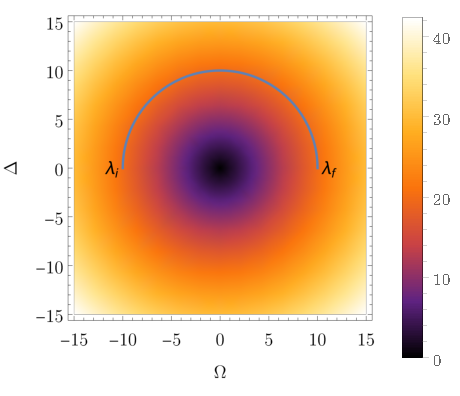
\includegraphics[scale=1.2]{../img/driving.pdf}
    \caption{Driving along the geodesic. $\lambda_i\equiv (\Omega_i,\Delta_i)$ and $\lambda_f\equiv (\Omega_f,\Delta_f)$ are initial and final parameters respective. Density plot shows the difference between Hamiltonian eigenvalues.}
    \label{fig:driving}
\end{figure}

\subsection{Derivation of the fidelity}
Because the Hamiltonian can be rewritten using Pauli matrices
\begin{equation}
    \HH(t) = 
        \begin{pmatrix}
         -s \cos (t \omega ) & s \sin (t \omega ) \\
         s \sin (t \omega ) & s \cos (t \omega ) \\
        \end{pmatrix}
        =\Delta(t)\sigma_x+ \Omega(t)\sigma_z= d(t).\mathbf{\hat{\bm\sigma}},
\end{equation}
for vector $\hat{\bm\sigma}\coloneqq (\hat\sigma_1,\hat\sigma_2,\hat\sigma_3)^T$.

One can see that changing from the \redd{original frame} with function $\ket{\psi}$ to \bluee{moving frame of reference}, with $\ket{\tilde\psi}$ (let's omit the final time dependence $\omega=\omega(T)$ for a while) is described as
\begin{equation}
    \redd{\psi(t)} \eqqcolon \expsp \bluee{\tilde\psi(t)}.
\end{equation}
This reflects the rotational symmetry of the system. The change of reference frame transforms Schr\"odinger equation as
\begin{equation}
    \begin{split}
        \redd{\HH(t)\psi(t)} &= i\redd{\psi'(t)}\\
        \redd{\HH(t)} \expsp\bluee{\tilde\psi(t)} &= i \expsp \left(\frac{i\omega\hat\sigma_y}{2}\right)\bluee{\tilde\psi(t)}+i\expsp\bluee{\tilde\psi'(t)}\\
        \underbrace{\left(\expsm \redd{\HH(t)}\expsp+ \frac{\omega}{2}\hat\sigma_y\right)}_{\bluee{\tilde H(t)}}\bluee{\tilde\psi(t)}&=i\bluee{\tilde\psi'(t)}.
    \end{split}
\end{equation}
From this one can equivalently solve the Fidelity problem in this new coordinate system.

Hamiltonian in the moving frame is
\begin{equation}
    \bluee{\tilde H}=\bluee{\begin{pmatrix}
        -s&-i\omega(T)/2\\
        i\omega(T)/2&s
    \end{pmatrix}},
\end{equation}
which is time independent and depends only on final time. The Schr\"odinger equation can now be easily solved using evolution operator
\begin{equation}
    \begin{split}
        \bluee{\UU(t)}=&e^{-i\bluee{\tilde H}t}\\
        =&\bluee{\begin{pmatrix}
            \cos \left(\frac{t}{2} q\right)+\frac{2 i s \sin \left(\frac{t}{2} q\right)}{q} & -\frac{\omega  \sin \left(\frac{t}{2} q\right)}{q} \\
            \frac{\omega  \sin \left(\frac{t}{2} q\right)}{q} & \cos \left(\frac{t}{2} q\right)-\frac{2 i s \sin \left(\frac{t}{2} q\right)}{q} \\
        \end{pmatrix}},
    \end{split}
    \label{eq:evolutionBlue}
\end{equation}
for $q\coloneqq\sqrt{4 s^2+\omega(T) ^2}$.

In the original frame we get the evolution of the state $\psi(0)$
\begin{equation}
    \redd{\psi(t)}=\expsp \bluee{\UU(t) \tilde\psi(0)} = \underbrace{\expsp \bluee{\UU}\expsm}_{\redd{\UU(t)}} \underbrace{\expsp \bluee{\tilde\psi(0)}}_{\redd{\psi(0)}}.
\end{equation}
The evolved wave-function the reads as
\begin{equation}
    \redd{\ket{\psi(t)}}=\redd{\begin{pmatrix}
        \cos \left(\frac{t}{2} q\right)+\frac{2 i s}{q} \cos (t \omega ) \sin \left(\frac{t}{2} q\right)\\
        \frac{\omega -2 i s\sin (t \omega )}{q}  \sin \left(\frac{t}{2} q\right)
    \end{pmatrix}}
\end{equation}
and the ground state
\begin{equation}
    \redd{\ket{0(t)}}=\redd{\mathcal{N}\begin{pmatrix}
        -\cot (\frac{t}{2}\omega(T))\\
        1
    \end{pmatrix}},
\end{equation}
for a normalization constant $\redd{\mathcal{N}}\coloneqq |\redd{\braket{0(t)|0(t)}}|^{-1}$.
Fidelity during the transport is then\footnote{If we calculated the fidelity in the \bluee{comoving frame}, we would get exactly one. This realization leads to the counter-diabatic driving.}
\begin{equation}
    F=\left|\redd{\braket{0(t)|\psi(t)}}\right|^2.
    \label{fid:definition}
\end{equation}

Explicit formula for fidelity in time $t$ and geodesic driving with final time $T$ is finally
\begin{equation}
    F(t,T)=\frac{\pi ^2 \left(\cos \left(t \sqrt{\frac{\pi ^2}{T^2}+4 s^2}\right)+1\right)+8 s^2 T^2}{2 \sin ^4\left(\frac{\pi  t}{2 T}\right) \left(4 s^2 T^2+\pi ^2\right) \left(\left| \cot \left(\frac{\pi  t}{2 T}\right)\right|^2+1\right)^2}.
    \label{eq:fidelitySimplified}
\end{equation}
The domain can be extended from $t\in(0,T)$ to $[0,T]$ for any $T\in[0,\infty]$, because 
$$
    \lim_{t\rightarrow 0}F=1\; ,\;\; \lim_{T\rightarrow 0}F=0.
$$

Sometimes the \emph{Infidelity}, defined as $F^*\coloneqq 1-F$, is used. It has a meaning of \emph{excitation probability during the transport}.


\subsection{Analysis of the infidelity formula}
Infidelity can be calculated by numerical evolution of Schr\"odinger equation, or from Eq. \ref{eq:fidelitySimplified}. Sometimes both solutions are plotted for comparison between numerical precision. 

For some fixed final time, the infidelity is an oscillating curve with values close to $0$, see the driving for final time $T=10$ on Fig. \ref{fig:infidelityTimePlot}. The \emph{final infidelity} (fidelity at $t=T$) dependence on final time $T$ can be seen on Fig. \ref{fig:infidelityTfPlot} and \ref{fig:infidelityTfPlotLog}.
\begin{figure}[H]
    \centering
    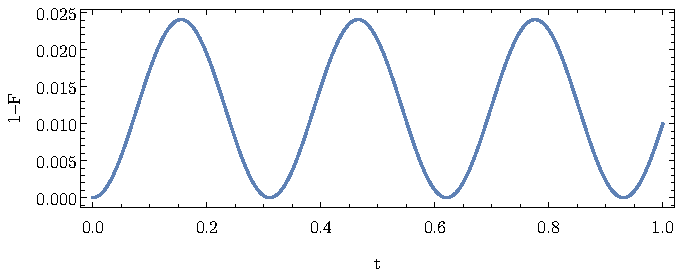
\includegraphics[scale=1.2]{../img/infidelityTimePlotGeod.pdf}
    \caption{Infidelity in time for final time $T=1$ for geodesical driving.}
  \label{fig:infidelityTimePlot}
\end{figure}

\vspace{-10pt}\begin{figure}[H]
    \centering
    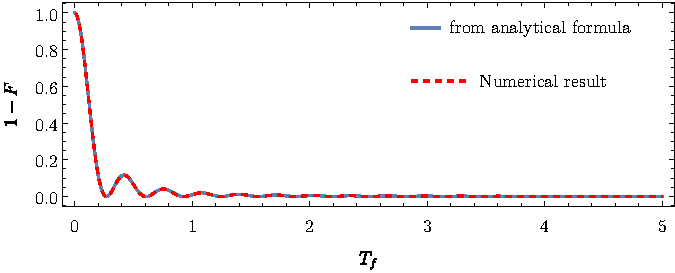
\includegraphics[scale=1.2]{../img/infidelityTfPlot.pdf}
    \caption{Final infidelity dependence on final time $T$ for geodesical driving.}
    \label{fig:infidelityTfPlot}
\end{figure}

\begin{figure}[H]
    \centering
    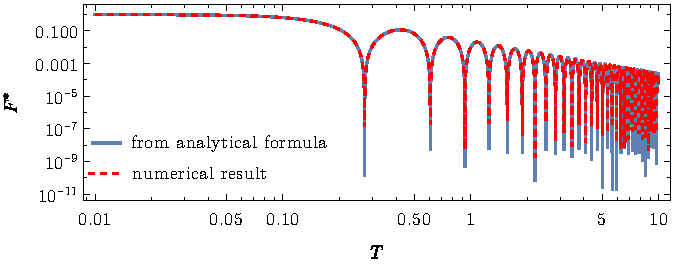
\includegraphics[scale=1.2]{../img/infidelityTfPlotLog.pdf}
    \caption{Infidelity dependence on final time in logarithmic scale. The difference in numerical precision of both methods can be seen in the spikes height. As it will be shown later, the spikes should go to zero, thus analytical formula has higher numerical precision.}
    \label{fig:infidelityTfPlotLog}
\end{figure}



From the fidelity formula \ref{eq:fidelitySimplified} goes that condition $F=1$ is equivalent to
\begin{equation}
    \cos \left(\sqrt{T_s^2+\pi ^2}\right)=1,
\end{equation}
for $T_s\coloneqq 2s T$. The solution to this equation is
\begin{equation}
    T_s=\sqrt{(2 \pi  k)^2-\pi ^2} \text{  for }k\in \mathbb{N},
    \label{eq:solutionT}
\end{equation}
see Fig. \ref{fig:fidelityZeros}. This implies that spikes on Fig. \ref{fig:infidelityTfPlotLog} have minimal value $1-F=0$. In addition, observe that their density is linear in $T$.
\begin{figure}[H]
    \centering
    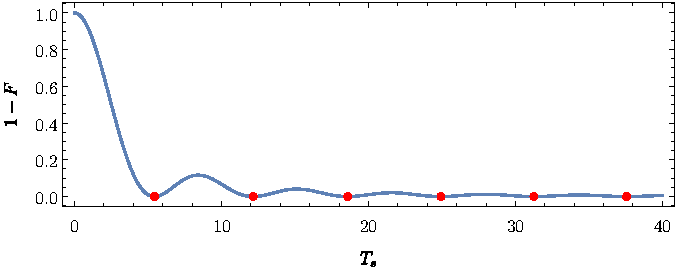
\includegraphics[scale=1.2]{../img/fidelityZeros.pdf}
    \caption{Rescaled final infidelity $T_s\coloneqq 2s T$ dependence on final time. Red points mark the condition $F=1$.}
    \label{fig:fidelityZeros}
\end{figure}


Fidelity as a function of time and final time can be seen in Fig. \ref{fig:dens3}. Note that only $t<T$ has physical meaning.

\begin{figure}[H]
    \centering
    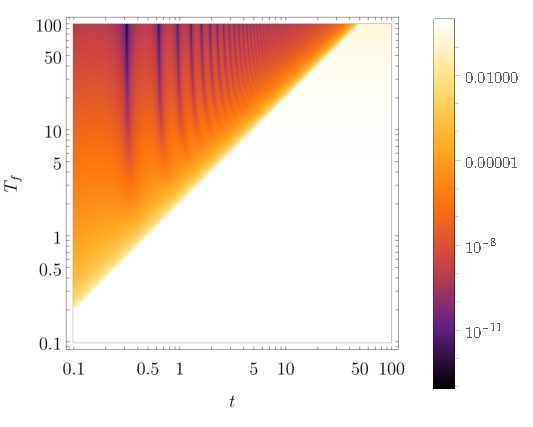
\includegraphics[scale=1.2]{../img/dens3.pdf}
    \caption{Fidelity dependence on time and final time in log-log scale. Note that only $t<T$ has physical meaning.}
    \label{fig:dens3}
\end{figure}

\subsection{Energy variance}
Another interesting quantity is the energy variance, specially because of Theorem \ref{thm:polkovnikov}. Evaluating the fidelity for geodesical driving gives a function of time $t$ and final time $T$
\begin{equation}
    \begin{split}        
        \delta E^2 =& \frac{s^2}{2 q^2}\Bigg[\Big[16 s^4+2 s^2 \left(\left(\omega ^2-8 s^2\right) \cos (2 t \omega )-8 \omega ^2 \cos ^2(t \omega ) \cos \left(t \sqrt{q}\right)\right)\\
        &+14 s^2 \omega ^2+\omega ^4\Big] -\omega ^2 \left(\left(2 s^2+\omega ^2\right) \cos (2 t \omega )-2 s^2\right) \cos \left(2 t q\right)\\
        & +8 s^2 \omega  q \sin (2 t \omega ) \sin \left(t q\right) + \omega ^3 q \sin (2 t \omega ) \sin \left(2 t q\right) \Bigg],
\end{split}
\end{equation}
see the definition of $q$ under Eq. \ref{eq:evolutionBlue}. The result of energy variance can be seen on Fig. \ref{fig:densVar}. Note that only $t<T$ has a physical meaning, therefore the dependence is smooth along the whole geodesical driving protocols.

\begin{figure}[H]
    \centering
    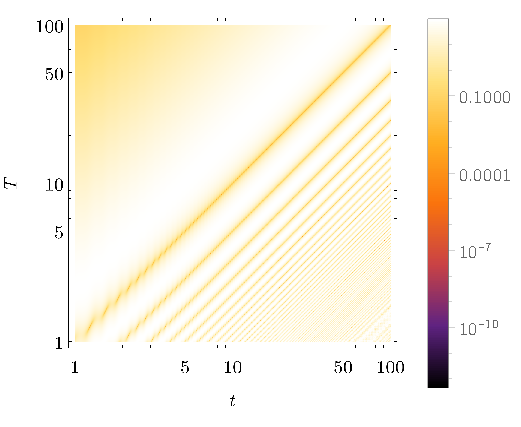
\includegraphics[scale=1.2]{../img/densVar.pdf}
    \caption{Energy variance for geodesical driving protocol, dependent on time $t$ and final time $T$. Driving occurs only in area $t<T$.}
    \label{fig:densVar}
\end{figure}

\newpage 
\section{Linear driving}
Another analytically solvable driving is defined using two scaling parameters $\Omega_{sc},\;\Delta_{sc}$, as 
\begin{equation}
    \Omega(t)=\Omega_{sc}\left(\frac{2t}{T}-1\right),\quad \Delta(t)=\Delta_{sc}, \;\;\text{ for } \Omega_{sc}=10, \Delta_{sc}=1,
    \label{eq:linearDrivingdef}
\end{equation}
see Fig. \ref{fig:driving1}. 
\begin{figure}[H]
    \centering
    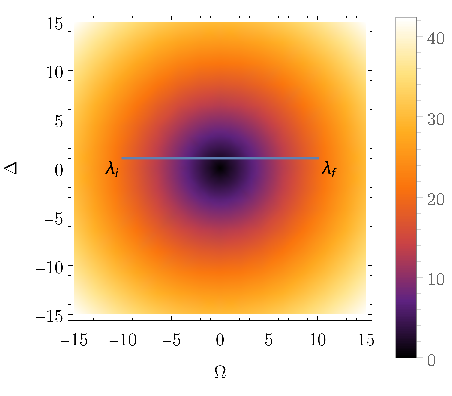
\includegraphics[scale=1.2]{../img/drivingLin.pdf}
    \caption{Driving along the linear path. $\lambda_i\coloneqq(-10;1)$ and $\lambda_f\coloneqq(10;1)$ are initial and final parameters respective. Density plot shows the difference between Hamiltonian eigenvalues.}
    \label{fig:driving1}
\end{figure}

From linear driving definition \ref{eq:linearDrivingdef} and energy dependence \ref{eq:energy} we have
\begin{equation}
    \dot \Delta(t)=0;\quad \Delta(t) \overset{\textcolor{gray}{\Delta(t)>0}}{=} \sqrt{\frac{E^2_{dif}(t)}{4}-\Omega^2(t)};\quad E_{dif}\coloneqq E_1-E_0.
\end{equation}
Substituting to Harmonic oscillator damping and frequency functions (Eq. \ref{eq:gammaDef} and \ref{eq:frequency}) we get 
\begin{align}
    \gamma(t) &= 0\\
    \omega^2(t)&=i\frac{2\Omega_{sc}}{T}+\frac{\Omega_{sc}}{4}\left(\frac{2t}{T}-1\right)^2+\frac{\Delta_{sc}^2}{4}=i\frac{2\Omega_{sc}}{T}+\frac{E^2_{dif}(t)}{4}.
    \label{eq:oscillationsLinear}
\end{align}
Corresponding differential equation of second order is
\begin{equation}
    a''(t)+\omega^2(t) a(t)=0,
\end{equation}
which is of \emph{Weber type}\footnote{https://mathworld.wolfram.com/WeberDifferentialEquations.html} with Parabolic Cylinder functions\footnote{https://mathworld.wolfram.com/ParabolicCylinderFunction.html} as a solution, see \cite{felipe}. 

\subsection{Dependence on time}
The fidelity in time can be seen on Fig. \ref{fig:infidelityTimePlotLin}. For $t\approx T/2$ Hamiltonian parameters change quickly which leads to fast state excitation. Then the Harmonic oscillator damping gets involved and oscillations are quickly going to zero, never disappearing entirely.

We can see that the final fidelity decreases with longer final time, which correctly leads to adiabatic driving, where $\lim_{T\rightarrow \infty} F^*=0$. For short final times we can observe so called quench, $\lim_{T\rightarrow 0} F^*=1$. The interesting phenomenon on this image are the oscillations around $t=T/2$, for which the frequency increases with longer final time. 

\begin{figure}[H]
    \centering 
    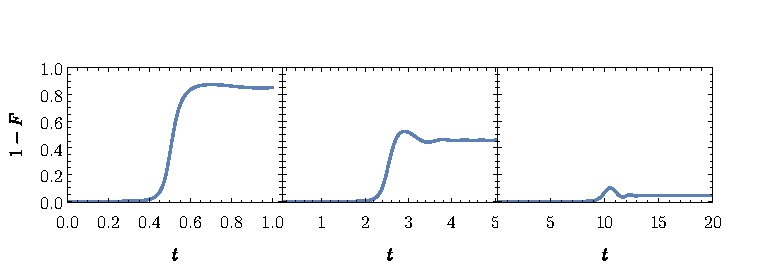
\includegraphics[scale=1.185]{../img/infidelityInTimePlot1.pdf}
    \caption{Infidelity in time for three final times $T\in\{1,5,20\}$ for the linear driving defined in \ref{eq:linearDrivingdef}.}
  \label{fig:infidelityTimePlotLin}
\end{figure}


Because in the Harmonic oscillator $\gamma(t)=0$, the oscillations of $a(t)$ are not damped. What we are observing is infidelity 
$$F^*(t)\coloneqq 1- |\braket{0(t)|\psi(t)}|^2 = 1-|\alpha(t)a(t)+\beta(t)b(t)|^2, $$
where the $\ket{\psi(t)}\eqqcolon(a,b)^T$ represents the evolved state and $\ket{0(t)}\eqqcolon(\alpha,\beta)^T$ evolved ground state in fixed eigenbasis $\mathcal{B}$. The ground state is not generally constant. In our case, the ground state described by Eq. \ref{eq:eigenvectors} and is slowly changing its value from the first element $\alpha$ to the second element $\beta$, see Fig. \ref{fig:zeroState}. This means that at the beginning of driving, the projection to the ground state selects $b(t)$. Then it's getting more influenced by $a(t)$ until almost only $a(t)$ influences the fidelity.
\begin{figure}[H]
    \centering
    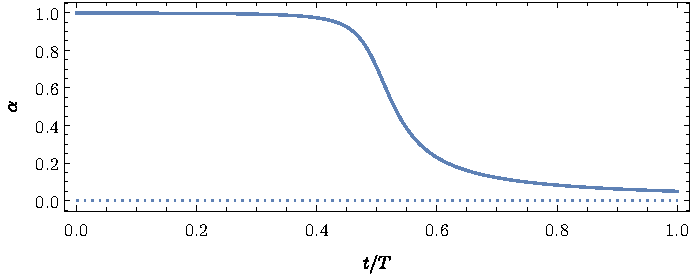
\includegraphics[scale=1.2]{../img/zeroState.pdf}
    \caption{Value of first element of the ground state vector $\alpha\equiv \ket{0(t)}^1$ during linear driving.}
    \label{fig:zeroState}
\end{figure}

Because of varying ground state during transport, the oscillations cannot be analyzed only from $\omega^2(t)$ described by Eq. \ref{eq:oscillationsLinear}. At the end of the driving we have 
\begin{equation}
   \frac{1}{N_+} \ket{0(t)}^1=\frac{E_0(t)+\Omega(t)}{\Delta(t)}\gg 1 =\frac{1}{N_+} \ket{0(t)}^2,
\end{equation}
leading to the \emph{fidelity at the end of the driving}
\begin{equation}
    F_{end}= \left|N_+ \left(
        \frac{E_0(t)+\Omega(t)}{\Delta(t)} a(t)+b(t)
        \right)\right|^2 \approx b^2(t),
\end{equation}
therefore when $t$ is getting close to $T$ the fidelity is oscillating with  harmonic oscillator frequency \ref{eq:frequency}.




\subsection{Final fidelity}
Because the oscillations after fast parameter change in the Hamiltonian never disappear entirely, we must observe these oscillations even at the final time. \emph{Final fidelity} (meaning the fidelity at $t=T$) has dependence on $T$ as can be seen in Fig. \ref{fig:infidelityTfPlotLogLinCombined}. Because after the final time $T\approx 120$ the values are so small, we can observe some fine structure of the fidelity, along with numerical error artifacts.
\begin{figure}[H]
    \centering
    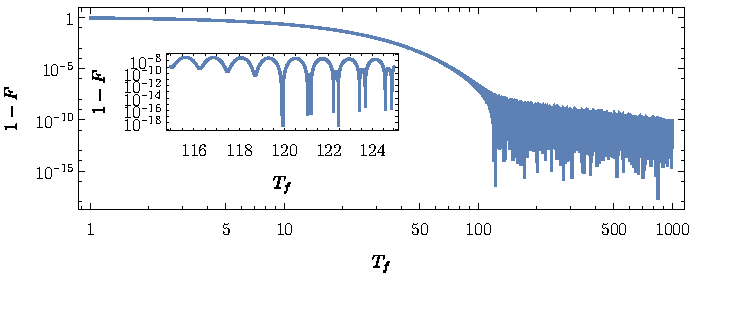
\includegraphics[scale=1.2]{../img/infidelityTfPlotLogLinCombined1.pdf}
    \caption{Final infidelity as a function of $T$ with zoom on the transitional part.}
    \label{fig:infidelityTfPlotLogLinCombined}
\end{figure}

First, the numerical precision of this calculation was found to be around $10^{-13}$. This means that the oscillations we see on Fig. \ref{fig:infidelityTfPlotLogLinCombined} are of physical origin with some additional numerical error. In fact these small oscillations are the remnants of the fast excitation during close approach of energy levels, see Fig. \ref{fig:infidelityTimePlotLin}. 



\subsubsection{Averaged final fidelity}
We can eliminate the effect of oscillations by averaging over time. For that we define the \emph{average final infidelity}
\begin{equation}
    \langle F^*\rangle_p(T) \coloneqq \frac{1}{(1-p) T}\int\limits_{(1-p) T}^{T} F^*(t)\d t.
\end{equation}
It turned out that averaging over 1 \% ($p=0.01$) or 10 \% ($p=0.1$) of the driving gave approximately the same results for long enough drivings ($T\overset{\sim}{>} 10$). The same result can be obtained from analytical continuation of the fidelity formula to $t\rightarrow  \infty$. This analytical continuation of harmonic oscillator solution leads to the Fidelity value around which the oscillations occur. The result of averaging can be seen on Fig. \ref{fig:infidCombined}.

Using this we can describe the driving using three regimes\footnote{The coefficient $p$ is assumed to be small enough not to cover the biggest oscillations after $t=T/2$ and big enough to average over sufficient number of oscillations. Approximately $p\in[0.6T,0.999T]$.}.
\begin{itemize}
    \item \emph{Exponential/fast-driving regime} — $\langle F^*\rangle_p= \exp(-\xi T)$, $\xi\in\R^+$
    \item \emph{transitional regime} — happens around \emph{critical time} $T_c$.
    \item \emph{Polynomial/close-adiabatic regime} — $\langle F^*\rangle_p\propto T^{-\kappa}$ for $\kappa\in \R^+$.
\end{itemize}

\begin{figure}[H]
    \centering
    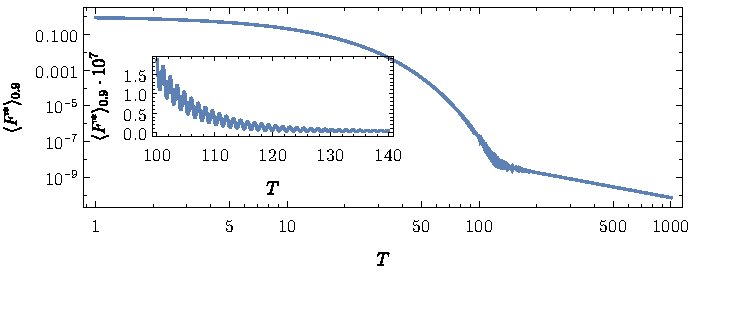
\includegraphics[scale=1.2]{../img/infidCombined1.pdf}
    \caption{Final infidelity as a function of $T$ in log-log scale wit linear scaled plot inserted.}
    \label{fig:infidCombined}
\end{figure}



The boundary between exponential and linear regime is not strict and can be seen on Fig. \ref{fig:dens2}, as transition between \emph{smooth} and \emph{chaotic} regimes. This happens around $t=T_c$. The fine structure, see Fig. \ref{fig:dens2Zoom}, is caused by the oscillatory character of the final fidelity. This would be smoothed out using the averaged final fidelity. The approximated dependence for final time was numerically estimated as
\begin{equation}
    T_c\overset{\sim}{\propto} \Delta_{sc}^{-2}.
\end{equation}


\begin{figure}[H]
    \centering 
    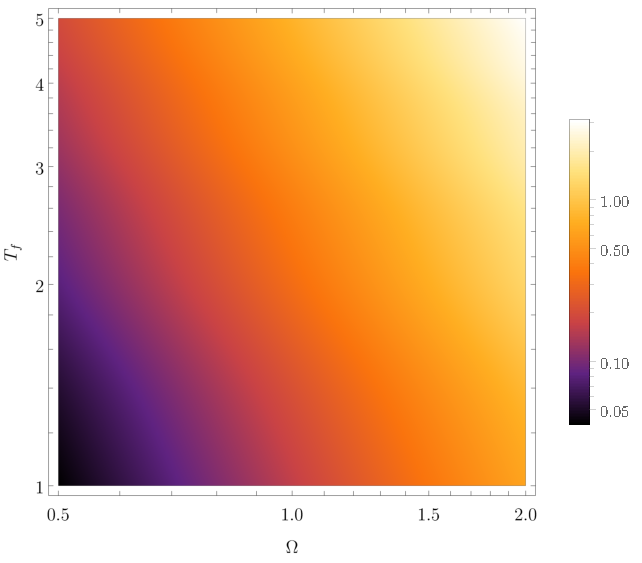
\includegraphics[scale=1.2]{../img/dens2.pdf}
    \caption{Final infidelity as a function of $\Delta$ and $T$ and its three regimes. Zoomed boundary between them can be seen on \ref{fig:dens2Zoom}.}
    \label{fig:dens2}
\end{figure}

\begin{figure}[H]
    \centering 
    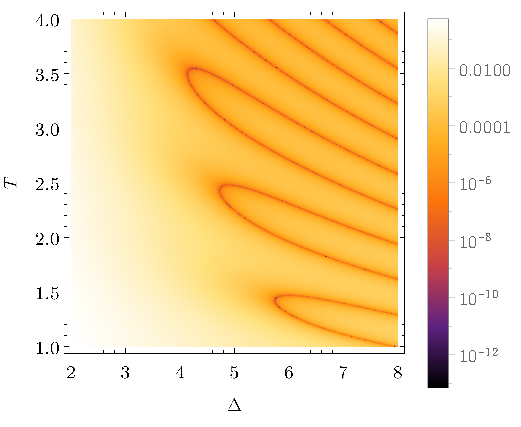
\includegraphics[scale=1.2]{../img/dens2Zoom.pdf}
    \caption{Fine structure of the boundary between fast-driving and adiabatic regimes of final infidelity.}
    \label{fig:dens2Zoom}
\end{figure}



To understand the infidelity oscillations, compare Fig. \ref{fig:undercritical} with \ref{fig:overcritical}. Here we see two regimes, one for $t<T_c$ and on for $T>T_c$. The important observation is that in the first case $F^*\neq 0$ for all $t>0$ and in the second case it touches zero periodically. The fidelity can be decomposed into a sum of two elements. Small oscillatory part, which can be explained by the theory of APT, and exponentially decreasing fidelity with final time, describable by Landau-Zener formula.

\begin{figure}[H]
    \centering
    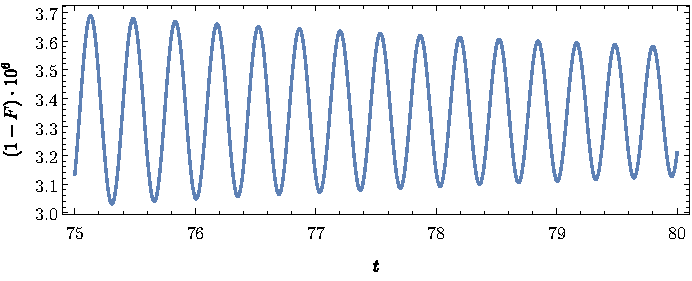
\includegraphics[scale=1.2]{../img/undercritical.pdf}
    \caption{Infidelity as function of time for fast-driving regime, $T=80<T_c$.}
    \label{fig:undercritical}
\end{figure}

\begin{figure}[H]
    \centering
    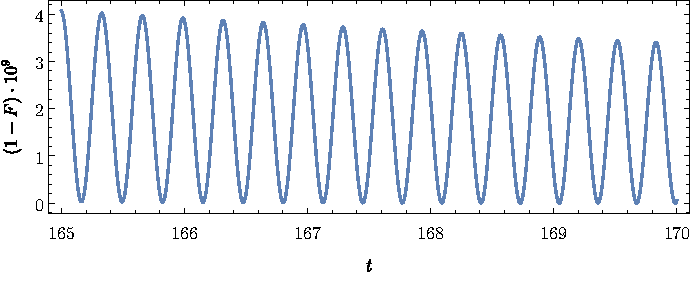
\includegraphics[scale=1.2]{../img/overcritical.pdf}
    \caption{Infidelity as function of time for close-adiabatic regime. $T=170>T_c$}
    \label{fig:overcritical}
\end{figure}

\subsubsection{Exponential and polynomial part, Landau-Zener and APT}
Landau-Zener-Stueckelberg theory provides the WKB approximation formula for the fidelity during some transport. Full form can be seen in \cite{nonadiabaticTransition}. In our case, only simplified theorem is needed. First let's review some definitions.

\begin{definition}[Diabatic coupling]
    Diabatic coupling functions are off-diagonal elements of two-level Hamiltonian. At avoided crossing, it is half of Hamiltonian eigenvalue difference,
    \begin{equation}
        A=\frac{E_2-E_1}{2}.
    \end{equation}
\end{definition}
\begin{definition}[Diabatic potential]
    Difference between Hamiltonian eigenvalues can be linearly approximated as
    \begin{equation}
        \Delta E\equiv E_1-E_0 \eqqcolon \alpha t
    \end{equation}
    Diabatic potential difference is the ratio
    \begin{equation}
        |\Delta F|\coloneqq \left|\frac{\alpha}{t}\right|.
    \end{equation}
\end{definition}

\begin{thm}[Landau-Zener-Stueckelberg (LZS) for linear driving]
    For 
    \begin{itemize}
        \item two level Hamiltonian
        \item with degeneracy in only one point,
        \item on the linear driving path in a parametric space
    \end{itemize}
    the fidelity can be described for times $t\in(0,T_c)$ as
    \begin{equation}
        F = \exp\left(-\frac{2 \pi A^2}{v|\Delta F|}\right),
        \label{eq:exponentialPart}
    \end{equation}
    for a \emph{diabatic coupling} $A$, and \emph{diabatic potential difference} $|\Delta F|$. 
\end{thm}

In our case, we have constant speed $v=1/T$, off-diagonal elements are also constant $A=\Delta_{sc}$, and the driving path is symmetric along $\Omega=0$ axis, leading to $|\Delta F|=2\Omega_i$.

The polynomial, or chaotic regime, can be explained using APT. It holds that
\begin{equation}
    \log(F^*)=\log(T^{-2})+\log\left(\sum_{i=1}^n |b_n^{(1)}(T)|^2\right),
    \label{eq:polynomialPart}
\end{equation}
for functions $b_n^{(1)}$ from Eq. \ref{eq:bnAPT}. For more details, see \cite{felipe}.

The LZS approximation can be seen on Fig. \ref{fig:landauCompare}. The LZS and APT approximations give the leading order in corresponding regimes (omitting the oscillations) and intersect at time $T_c$. In fact these two parts are not only the good approximation on both intervals, but if added together, they represent the whole fidelity curve with very high precision. It might not give a good mathematical meaning to add these two solutions together. But because the APT gives the infidelity of order $10^{-9}$, it creates negligible error. The advantage is that by this process one gets suitable approximation for the transitional regime.


\begin{figure}[H]
    \centering 
    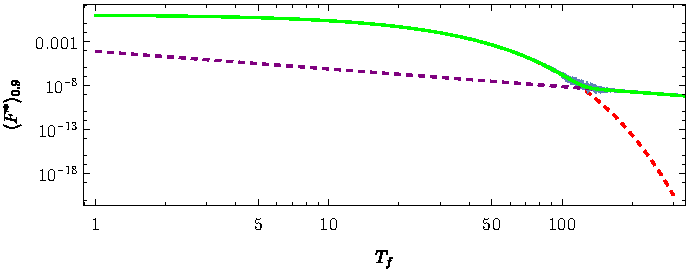
\includegraphics[scale=1.2]{../img/landauCompare.pdf}
    \caption{Fidelity as a function of driving final time, approximated by the \green{sum (green)} of \red{Landau-Zener (red, dashed)} and \textcolor{purple}{APT (purple, dashed)}}
    \label{fig:landauCompare}
\end{figure}
% \subsection{Multiparametric behavior}
% The critical time $T_c$ is the point where the fidelity dependence on final time becomes polynomial. We have shown that 
% \begin{equation}
%     \text{for}\begin{cases}
%         T<T_c \\
%         T>T_c 
%     \end{cases}\text{the fidelity oscillate with amplitude } A \text{ is }
%     \begin{cases}
%         A<1-F_{final}\\
%         A>1-F_{final}
%     \end{cases}.
% \end{equation}




\subsection{Summary of linear driving}
Now we understand all results separately, let's put it all together. On Fig. \ref{fig:AllInOne} the most important results can be seen. The difference in the close adiabatic regime and fast regime at the end of the driving is if $F^*=0$. The chaotic regime is below $t=T$ line for $T<T_c$ and the chaotic cone is crossing this line around $t=T_c$.

\begin{figure}[H]
    \centering 
    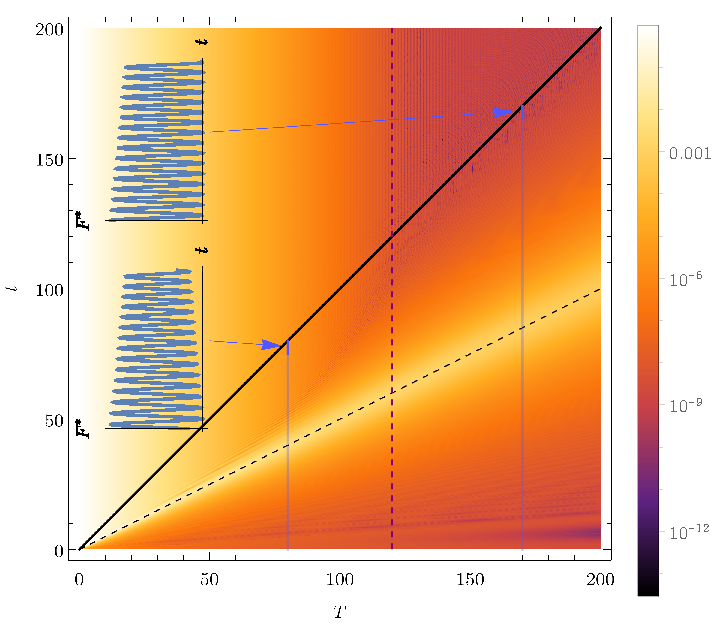
\includegraphics[scale=1.2]{../img/allInOne.pdf}
    \caption{Fidelity dependence for linear driving with $\Delta=1$. Black line marks $t=T$, dashed black line $t=T/2$ and \redd{purple} dashed line is the approximate value of $T_c$. \bluee{Blue} lines marks driving from Fig. \ref{fig:undercritical}, \ref{fig:overcritical}, visualizing the final times of the driving.}
    \label{fig:AllInOne}
\end{figure}









\newpage
\subsection{Energy variance}
Analogically to the geodesical driving, one might be interested in energy variance. In the linear driving case, the analytical formula is more complicated and only numerical result are displayed here. On Fig. \ref{fig:densVariance} the energy variance is plotted as a function of time and final time.
\begin{figure}[H]
    \centering
    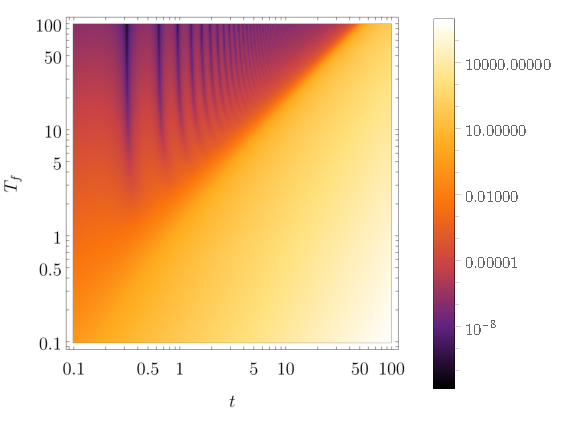
\includegraphics[scale=1.2]{../img/densVariance.pdf}
    \caption{Energy variance for $\Delta_{sc}=0.2$ for linear driving. Note that only $t<T$ has physical meaning.}
    \label{fig:densVariance}
\end{figure}
















